\documentclass[t]{beamer}

\usetheme{default}
\usebackgroundtemplate{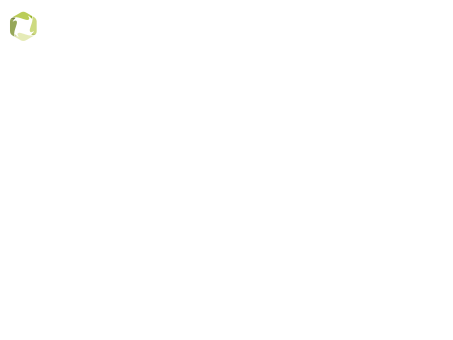
\includegraphics[width=\paperwidth]
                                       {../cpeb_bkground_topleftlogo.pdf}}

\setbeamertemplate{frametitle}{
  \centering\vspace{1mm}\insertframetitle\par\vspace{3mm}
}

\usepackage[style=nature,
            hyperref,
            backend=biber,
            isbn=false,
            doi=false,
            url=false,
            date=year,
            maxbibnames=3
           ]{biblatex}

\bibliography{kdm.bib}

\title{\texttt{kWIP}: The k-mer Weighted Inner Product}
\subtitle{Estimating genetic similarity of sequencing runs}
\author{Kevin Murray}
\institute{PhD Candidate\\ Borevitz Lab, ANU}
\date{2016-11-02}

\usefonttheme{serif}

% Remove Figure: prefix from captions
\usepackage{caption}
\captionsetup[figure]{labelformat=empty}

\begin{document}

{
\usebackgroundtemplate{
\includegraphics[width=\paperwidth]{../cpeb_bkground_centered.pdf}}
\begin{frame}
  \titlepage
  \vfill
\end{frame}
}

\begin{frame}{Motivation}
  \begin{figure}
    \centering
    \includegraphics[width=0.45\textwidth]{img/euc.jpg}
    \includegraphics[width=0.4\textwidth]{img/albens.jpg}
  \end{figure}
\end{frame}

\begin{frame}{Collection Re-structuring}
  \begin{itemize}
    \item Collect 100s or 1,000s of natural samples
    \item ``First look'' at genetic relatedness
    \begin{itemize}
      \item Assert replicates cluster, detect mixups
      \item Carry best samples to detailed analysis
    \end{itemize}
  \end{itemize}
  \begin{center}
    \includegraphics<1>[width=\textwidth]{img/restruct-1}
    \includegraphics<2>[width=\textwidth]{img/restruct-2}
    \includegraphics<3>[width=\textwidth]{img/restruct-3}
    \begin{itemize}
      \item[]<1-3> \tiny{after \textcite{brachi_genome-wide_2011}}
    \end{itemize}
  \end{center}
\end{frame}


\begin{frame}{(Initial) Genetic Similarity Estimation}
  \begin{itemize}
    \item Initial genetic analyses inspect
      \begin{itemize}
        \item Outgroups (widest relationships)
        \item Replicates
        \item Mix-ups
        \item Broad groupings
      \end{itemize}
    \item Current genetic similarity, \textit{not evolutionary history}
  \end{itemize}
  \begin{figure}
    \centering
    \includegraphics[width=\textwidth]{img/cross-scale.png}
  \end{figure}
  \tiny{after \textcite{peterson_double_2012}}
\end{frame}


\begin{frame}[c]{Genetic Similarity Estimation -- Algorithms}
  \begin{itemize}
    \item Efficient algorithms to analyse large-scale genomic data
    \begin{itemize}
      \item Reference \& alignment free: \textit{less bias, de novo}
      \item Platform/protocol agnostic: \textit{future proof}
      \item Computationally efficient: \textit{not the bottleneck}
    \end{itemize}
  \end{itemize}
\end{frame}

\begin{frame}{Alignment-free Sequence Comparison}
  \begin{itemize}
    \item Many existing metrics, and tools
    \begin{itemize}
      \item $D2$ and related statistics
      \item \texttt{spaced} and other spaced-word approaches
        \autocite{morgenstern_estimating_2015,leimeister_fast_2014}
      \item \texttt{Cnidaria} and other Jaccard index approaches
        \autocite{aflitos_cnidaria:_2015}
      \item \texttt{mash} and other MinHash approaches
        \autocite{ondov_fast_2015}
    \end{itemize}
    \item Most require assembled gene/genome sequence
    \item \textbf{Most assume evolutionary history between samples}
  \end{itemize}
  \begin{figure}
    \centering
    \includegraphics[width=0.4\textwidth]{img/aln.jpg}
  \end{figure}
\end{frame}


\begin{frame}{Presenting \texttt{kWIP}}
  \begin{itemize}
    \item $k$-mer based \textit{de novo} genetic similarity estimator
    \item Produces a distance matrix from raw NGS reads
    \item Uses Weighted Inner Product between $k$-mer counts
  \end{itemize}
  \begin{center}
    \includegraphics[width=\textwidth]{img/kwip-overview.png}
  \end{center}
\end{frame}

\begin{frame}{\texttt{kWIP} Algorithm}
  \begin{itemize}
    \item Count each sample's $k$-mers probabilistically (\texttt{khmer})
    \item Calculate information content of each $k$-mer
    \item Compute each pairwise distance using weighed inner product (WIP)
  \end{itemize}
  \begin{center}
    \includegraphics[width=0.5\textwidth]{img/sketch_aggregation.pdf}
    \includegraphics[width=0.37\textwidth]{img/shanent.pdf}
  \end{center}
\end{frame}

\begin{frame}{\texttt{kWIP} -- Software}
  \begin{itemize}
    \item Uses \texttt{khmer} for $k$-mer counting
    \item Parallelised with OpenMP
    \item GNU GPL licensed, \texttt{C++11} source code on GitHub
    \item Precompiled binaries provided
    \item Documentation \& tutorials online
  \end{itemize}
  \begin{figure}
    \centering
    \includegraphics[width=0.7\textwidth]{img/kwip-doc-screenshot.png}
  \end{figure}
\end{frame}

\begin{frame}{\texttt{kWIP} Case Studies}
  \begin{itemize}
    \item Rice genomes project
        \autocite{the_3000_rice_genomes_project_3000_2014}
      \begin{itemize}
        \item 3000 rice varieties (25k runs)
        \item $\approx 2$-fold sequencing per run
      \end{itemize}
    \item Population genomics -- Chlamydomonas \autocite{flowers_whole-genome_2015}
      \begin{itemize}
        \item High-coverage sequencing of 20 wild \& lab strains
      \end{itemize}
    \item Rice root-associated microbiome metagenomics
      \begin{itemize}
        \item Shotgun sequencing of root-soil interface
      \end{itemize}
    \item Simulation
      \begin{itemize}
        \item Fake population genome sequencing studies
      \end{itemize}
  \end{itemize}
\end{frame}

\begin{frame}{Replicate and Subspecies Clustering}
  \begin{itemize}
    \item Set of 96 rice runs from 16 samples, 6 tech reps.
    \item $\approx 3$-fold sequencing per run
    \item Expectations:
      \begin{itemize}
        \item All runs cluster into samples of 6 reps
        \item Big split between 2 major groups (Indica, Japonica)
      \end{itemize}
    \item Recover known grouping w/ \texttt{kWIP}, not w/ unweighted IP
    \item Took 6 hours on 16 CPU, 64GB RAM supercomputer node
    \item Similar patterns observed over 100s of similar subsets
  \end{itemize}
\end{frame}

\begin{frame}
  \begin{center}
    \includegraphics<1>[width=0.6\textwidth]{img/dendro-wip.png}
    \includegraphics<2>[width=0.6\textwidth]{img/dendro-ip.png}
  \end{center}
\end{frame}

\begin{frame}{Chlamydomonas}
  \begin{columns}[t]
    \begin{column}{0.5\textwidth}
        \begin{itemize}
          \item Avoid reference bias with ``leftover assembly''
              \autocite{flowers_whole-genome_2015}
            \begin{itemize}
              \item Sequence \textit{very} deep ($> 200$x)
              \item Map to reference
              \item Assemble umapped reads
              \item Map to reference + leftovers
              \item Call variants
              \item \texttt{SNPrelate} + PCA
            \end{itemize}
        \end{itemize}
    \end{column}
    \begin{column}{0.5\textwidth}
      \begin{center}
        \includegraphics[width=\textwidth]{img/flowers.png}
        \begin{itemize}
          \item[] \tiny{\textit{``Sample CC-4414 (red) is hidden behind the cluster of laboratory
            strains (light blue)''}}
        \end{itemize}
      \end{center}
    \end{column}
  \end{columns}
\end{frame}

\begin{frame}{Chlamydomonas -- with \texttt{kWIP}}
  \begin{itemize}
    \item Download SRA files
    \item Count $k$-mers
    \item Run \texttt{kWIP}
  \end{itemize}
  \begin{figure}
    \centering
    \includegraphics[width=0.5\textwidth]{img/flowers.png}
    \includegraphics[width=0.48\textwidth]{img/chlamy.pdf}
  \end{figure}
\end{frame}

\begin{frame}{Metagenomes}
  \begin{figure}
    \centering
    \includegraphics[width=0.5\textwidth]{img/greenhouse_edwards.png}
    \includegraphics[width=0.5\textwidth]{img/greenhouse_nw.pdf}
  \end{figure}
\end{frame}

\begin{frame}{Simulation}
  \begin{itemize}
    \item Perform simulated sequencing experiment (50 times):
    \begin{itemize}
      \item Simulate natural population structure
      \item Simulate sample genomes
      \item Simulate sequencing runs (with random variation)
      \item Sketch reads, \texttt{kWIP}
      \item Compare \texttt{kWIP} results to known truth
      \item Spearmans Rank Correlation ($\rho$),  ``Performance''
    \end{itemize}
    \item kWIP quantitatively outperforms unweighted equivalent
      \begin{itemize}
        \item Performs reasonably at low-moderate coverage
        \item Performance stable across scale of variation
      \end{itemize}
  \end{itemize}
\end{frame}

\begin{frame}{Performance vs Coverage}
  \begin{figure}
    \centering
    \includegraphics[width=0.7\textwidth]{img/coverage-vs-rho_50x.pdf}
  \end{figure}
\end{frame}

\begin{frame}{Performance vs Mean pairwise distance ($\pi$)}
  \begin{figure}
    \centering
    \includegraphics[width=0.7\textwidth]{img/pi-vs-performance.pdf}
  \end{figure}
\end{frame}

\begin{frame}{\texttt{kWIP} Summary}
  \begin{itemize}
    \item \texttt{kWIP} is implemented, no known bugs
    \item Publicly available at \url{github.com/kdmurray91/kwip}
    \item We show the utility of \texttt{kWIP}
    \item Publication in review at PLoS Comp. Biol. (\url{bit.do/kwip})
    \item Version 2 on the way
    \begin{itemize}
      \item MPI parallel
      \item More metrics
      \item Even faster
    \end{itemize}
  \end{itemize}
\end{frame}

\begin{frame}{Thanks}
  \begin{columns}
    \begin{column}{0.7\textwidth}
      \begin{itemize}
        \item Norman Warthmann, Justin Borevitz
        \item Christfried Webers, Cheng Soon Ong
        \item Sylvain For\^{e}t
        \item $AB^3ACBS$ Organisers and Yourselves
      \end{itemize}
    \end{column}
    \begin{column}{0.2\textwidth}
      \begin{figure}
        \centering
        \includegraphics[width=\textwidth]{img/link.png}
      \end{figure}
    \end{column}
  \end{columns}
  \begin{figure}
    \centering
    \includegraphics[width=0.7\textwidth]{img/lab.jpg}
  \end{figure}
\end{frame}

\begin{frame}[shrink=40]{}
  \printbibliography
  \vfill
  .
\end{frame}

\end{document}
